% This file was created with tikzplotlib v0.10.1.
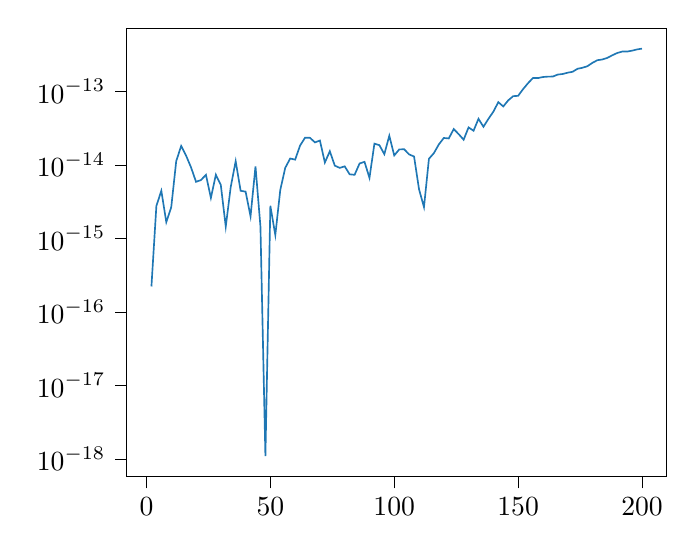
\begin{tikzpicture}

\definecolor{darkgray176}{RGB}{176,176,176}
\definecolor{steelblue31119180}{RGB}{31,119,180}

\begin{axis}[
log basis y={10},
tick align=outside,
tick pos=left,
x grid style={darkgray176},
xmin=-7.9, xmax=209.9,
xtick style={color=black},
y grid style={darkgray176},
ymin=5.77616866396572e-19, ymax=7.21000033819287e-13,
ymode=log,
ytick style={color=black},
ytick={1e-20,1e-19,1e-18,1e-17,1e-16,1e-15,1e-14,1e-13,1e-12,1e-11},
yticklabels={
  \(\displaystyle {10^{-20}}\),
  \(\displaystyle {10^{-19}}\),
  \(\displaystyle {10^{-18}}\),
  \(\displaystyle {10^{-17}}\),
  \(\displaystyle {10^{-16}}\),
  \(\displaystyle {10^{-15}}\),
  \(\displaystyle {10^{-14}}\),
  \(\displaystyle {10^{-13}}\),
  \(\displaystyle {10^{-12}}\),
  \(\displaystyle {10^{-11}}\)
}
]
\addplot [semithick, steelblue31119180]
table {%
2 2.22048945968886e-16
4 2.77555777332113e-15
6 4.44089209850063e-15
8 1.66533453693773e-15
10 2.66453525910038e-15
12 1.12132525487141e-14
14 1.80966353013901e-14
16 1.33226762955019e-14
18 9.2148511043888e-15
20 5.88418203051333e-15
22 6.21724893790088e-15
24 7.32747196252603e-15
26 3.5527136788005e-15
28 7.32747196252603e-15
30 5.32907051820075e-15
32 1.44329035552918e-15
34 4.9960036108132e-15
36 1.12132525487141e-14
38 4.4408925220171e-15
40 4.32986979603811e-15
42 1.99840207959999e-15
44 9.54791801177635e-15
46 1.44329003789182e-15
48 1.09331222276428e-18
50 2.77555798507936e-15
52 1.11022334226251e-15
54 4.55191440096314e-15
56 9.10382880192628e-15
58 1.22124532708767e-14
60 1.17683640610267e-14
62 1.83186799063151e-14
64 2.34257058195908e-14
66 2.33146835171283e-14
68 2.02060590481778e-14
70 2.14273043752655e-14
72 1.0769163338864e-14
74 1.53210777398272e-14
76 9.76996261670138e-15
78 9.10382880192628e-15
80 9.54791801177635e-15
82 7.43849426498855e-15
84 7.32747196252603e-15
86 1.04360964314765e-14
88 1.0991207943789e-14
90 6.66133814775094e-15
92 1.94289029309402e-14
94 1.85407245112401e-14
96 1.3988810110277e-14
98 2.48689957516035e-14
100 1.34336985979644e-14
102 1.62092561595273e-14
104 1.63202784619898e-14
106 1.38777878078145e-14
108 1.29896093881143e-14
110 4.66293670342566e-15
112 2.66453547085861e-15
114 1.21014309684142e-14
116 1.4432899320127e-14
118 1.89848137210902e-14
120 2.32036612146658e-14
122 2.28705943072782e-14
124 3.06421554796543e-14
126 2.62012633811537e-14
128 2.19824158875781e-14
130 3.23074900165921e-14
132 2.90878432451791e-14
134 4.22994972382185e-14
136 3.29736238313671e-14
138 4.21884749357559e-14
140 5.28466159721575e-14
142 7.1276318180935e-14
144 6.22835116814713e-14
146 7.53841433720481e-14
148 8.59312621059871e-14
150 8.69304628281498e-14
152 1.07136521876328e-13
154 1.29118937763906e-13
156 1.51989532071184e-13
158 1.51434420558871e-13
160 1.56541446472147e-13
162 1.5842882561401e-13
164 1.5887291482386e-13
166 1.68975944347949e-13
168 1.72195591119362e-13
170 1.791899961745e-13
172 1.84630088995164e-13
174 2.02837746599016e-13
176 2.09277040141842e-13
178 2.19935181178244e-13
180 2.44249065417534e-13
182 2.65121258280487e-13
184 2.71116462613463e-13
186 2.8510527272374e-13
188 3.09197112358106e-13
190 3.32289751270309e-13
192 3.47388784405211e-13
194 3.47166739800286e-13
196 3.574918139293e-13
198 3.71369601737115e-13
200 3.80917519748891e-13
};
\end{axis}

\end{tikzpicture}
